%% ----------------------------------------------------------------
%% Thesis.tex
%% ---------------------------------------------------------------- 
\documentclass[sotoncolour]{uosthesis}      % Use the Thesis Style with custom link colour
\graphicspath{{Figures/}}   % Location of your graphics files
\usepackage[round]{natbib}            % Use Natbib style for the refs.
\setcitestyle{numbers}
\usepackage{bibentry}          % Use bibentry for prepublished works
\nobibliography*               % Use bibentry for prepublished works
\usepackage{attrib}            % Use the attrib package for quotations
\hypersetup{colorlinks=true}   % Set to false for black/white printing
%% ----------------------------------------------------------------
%% Definitions.tex
%% ---------------------------------------------------------------- 
\RequirePackage{mathtools}
\RequirePackage{xparse}
\RequirePackage{pgffor}
\RequirePackage{ifthen}
\RequirePackage{amssymb}
\RequirePackage{xspace}


\newcommand{\BibTeX}{{\rm B\kern-.05em{\sc i\kern-.025em b}\kern-.08em T\kern-.1667em\lower.7ex\hbox{E}\kern-.125emX}}

%% People
\newcounter{address}
\setcounter{address}{1}
\renewcommand{\theaddress}{\textsuperscript{\fnsymbol{address}}}
\newcommand{\address}[1]{\refstepcounter{address}\theaddress#1\\}
\newcommand{\Name}[3]{\texorpdfstring{\href{mailto:#3}{#2}#1}{#2}\xspace}
\newcommand{\SteveRGunn}[1]{\Name{#1}{Steve R. Gunn}{S.R.Gunn@ecs.soton.ac.uk}}

%% Dingbats
\newcommand{\tick}{\ding{51}}
\newcommand{\cross}{\ding{55}}

%% Calculus
\newcommand{\pd}[2]{\ensuremath{\frac{\partial #1}{\partial #2}}\xspace}
\newcommand{\fd}[2]{\ensuremath{\frac{d #1}{d #2}}\xspace}
\newcommand{\dint}{\ensuremath{\int\!\!\!\int}\xspace}
\newcommand{\tint}{\ensuremath{\int\!\!\!\int\!\!\!\int}\xspace}

%% Math Sets
\newcommand{\Q}[1]{\ensuremath{\mathbb{#1}}\xspace}
\newcommand{\R}{\Q{R}}

%% Matrix, Vector
\newcommand{\V}[1]{\ensuremath{\boldsymbol{#1}}\xspace}
\newcommand{\M}[1]{\ensuremath{\boldsymbol{#1}}\xspace}
\newcommand{\0}{\V{0}}
\newcommand{\1}{\V{1}}
\newcommand{\I}{\M{I}}

%% Math Functions
\newcommand{\F}[1]{\ensuremath{\mathrm{#1}}\xspace}
\newcommand{\sgn}{\F{sgn}}
\newcommand{\tr}{\F{trace}}
\newcommand{\diag}{\F{diag}}

%% Math Names
\newcommand{\N}[1]{\ensuremath{\mathit{#1}}\xspace}

%% Data
\newcommand{\mc}[1]{\ensuremath{\mathcal{#1}}\xspace}
\newcommand{\Hyp}{\mc{H}}
\newcommand{\D}{\mc{D}}

%% Kernel
\newcommand{\K}{\M{K}}
\newcommand{\eins}{\texorpdfstring{\ensuremath{\epsilon}}{\textepsilon}-insensitive\xspace}
\newcommand{\e}{\ensuremath{\epsilon}\xspace}
\newcommand{\Bxi}{\ensuremath{\boldsymbol{\xi}}\xspace}
\newcommand{\Kanova}{\ensuremath{\mathit{K_{ANOVA}}}\xspace}
\newcommand{\Kspline}{\ensuremath{\mathit{K_{spline}}}\xspace}

%% Bayesian
\newcommand{\MP}{\ensuremath{\mathit{{\scriptscriptstyle \hspace{-1.5pt}M\hspace{-1.5pt}P}}}\xspace}
\newcommand{\ML}{\ensuremath{\mathit{{\scriptscriptstyle \hspace{-1.5pt}M\hspace{-1.5pt}L}}}\xspace}
\newcommand{\Qw}{\ensuremath{Q_{\w}(\w)}\xspace}
\newcommand{\Qa}{\ensuremath{Q_{\Ba}(\Ba)}\xspace}
\newcommand{\Qb}{\ensuremath{Q_{\beta}(\beta)}\xspace}
\newcommand{\wMPab}{\ensuremath{\w_{\MP|\bar {\Ba},\bar \beta}}\xspace}
\newcommand{\wMP}{\ensuremath{\w_{\MP}}\xspace}
\newcommand{\yMP}{\ensuremath{y_{\MP}}\xspace}
\newcommand{\BaMP}{\ensuremath{\Ba_{\hspace{1pt}\MP}}\xspace}
\newcommand{\aMP}{\ensuremath{\alpha_{\hspace{1pt}\MP}}\xspace}
\newcommand{\bMP}{\ensuremath{\beta_{\hspace{1pt}\MP}}\xspace}
\newcommand{\Sab}{\ensuremath{\M{\Sigma}_{\bar \Ba,\bar \beta}}\xspace}
\newcommand{\Ba}{\ensuremath{\boldsymbol{\alpha}}\xspace}
\newcommand{\Bb}{\ensuremath{\boldsymbol{\beta}}\xspace}
\newcommand{\Bm}{\ensuremath{\boldsymbol{\mu}}\xspace}
\newcommand{\BL}{\ensuremath{\boldsymbol{\Lambda}}\xspace}
\newcommand{\BPhi}{\ensuremath{\boldsymbol{\Phi}}\xspace}
\newcommand{\SMP}{\ensuremath{\M{\Sigma}_{\MP}}\xspace}

\newcommand{\Pa}{\ensuremath{P(\alpha|\mathcal{H})}\xspace}
\newcommand{\Pb}{\ensuremath{P(\beta|\mathcal{H})}\xspace}
\newcommand{\Pab}{\ensuremath{P(\alpha,\beta|\mathcal{H})}\xspace}
\newcommand{\Pw}{\ensuremath{P(\w|\mathcal{H})}\xspace}
\newcommand{\PD}{\ensuremath{P(\D|\mathcal{H})}\xspace}
\newcommand{\PwIa}{\ensuremath{P(\w|\alpha,\mathcal{H})}\xspace}
\newcommand{\PDIwb}{\ensuremath{P(\D|\w,\beta,\mathcal{H})}\xspace}
\newcommand{\PDwab}{\ensuremath{P(\D,\w,\alpha,\beta|\mathcal{H})}\xspace}
\newcommand{\PDIw}{\ensuremath{P(\D|\w,\mathcal{H})}\xspace}
\newcommand{\PwID}{\ensuremath{P(\w|\D,\mathcal{H})}\xspace}
\newcommand{\PwabID}{\ensuremath{P(\w,\alpha,\beta|\D,\mathcal{H})}\xspace}

\newcommand{\PanH}{\ensuremath{P(\alpha)}\xspace}
\newcommand{\PbnH}{\ensuremath{P(\beta)}\xspace}
\newcommand{\PabnH}{\ensuremath{P(\alpha,\beta)}\xspace}
\newcommand{\PwnH}{\ensuremath{P(\w)}\xspace}
\newcommand{\PDnH}{\ensuremath{P(\D)}\xspace}
\newcommand{\PwIanH}{\ensuremath{P(\w|\alpha)}\xspace}
\newcommand{\PDIwbnH}{\ensuremath{P(\D|\w,\beta)}\xspace}
\newcommand{\PDwabnH}{\ensuremath{P(\D,\w,\Ba,\beta)}\xspace}
\newcommand{\PDIwnH}{\ensuremath{P(\D|\w)}\xspace}
\newcommand{\PwIDnH}{\ensuremath{P(\w|\D)}\xspace}
\newcommand{\PwabIDnH}{\ensuremath{P(\w,\alpha,\beta|\D)}\xspace}

\newcommand{\PDwBab}{\ensuremath{P(\D,\w,\Ba,\beta|\mathcal{H})}\xspace}
\newcommand{\PwIBa}{\ensuremath{P(\w|\Ba,\mathcal{H})}\xspace}
\newcommand{\PBab}{\ensuremath{P(\Ba,\beta|\mathcal{H})}\xspace}
\newcommand{\PwBabID}{\ensuremath{P(\w,\Ba,\beta|\D,\mathcal{H})}\xspace}

\newcommand{\PBanH}{\ensuremath{P(\Ba)}\xspace}
\newcommand{\PwIBanH}{\ensuremath{P(\w|\Ba)}\xspace}

%% Snakes
\newcommand{\Esnake}{\ensuremath{\mathit{E_{snake}}}\xspace}
\newcommand{\Eimage}{\ensuremath{\mathit{E_{image}}}\xspace}
\newcommand{\Econt}{\ensuremath{\mathit{E_{cont}}}\xspace}
\newcommand{\Ecurv}{\ensuremath{\mathit{E_{curv}}}\xspace}
\newcommand{\Eint}{\ensuremath{\mathit{E_{int}}}\xspace}
\newcommand{\Eext}{\ensuremath{\mathit{E_{ext}}}\xspace}
\newcommand{\Eterm}{\ensuremath{\mathit{E_{term}}}\xspace}
\newcommand{\Eline}{\ensuremath{\mathit{E_{line}}}\xspace}
\newcommand{\Eedge}{\ensuremath{\mathit{E_{edge}}}\xspace}
\newcommand{\Econ}{\ensuremath{\mathit{E_{con}}}\xspace}
\newcommand{\Eangle}{\ensuremath{\mathit{E_{angle}}}\xspace}
\newcommand{\Elshape}{\ensuremath{\mathit{E_{lshape}}}\xspace}
\newcommand{\Eedgedir}{\ensuremath{\mathit{E_{edgedir}}}\xspace}
\newcommand{\Emodel}{\ensuremath{\mathit{E_{model}}}\xspace}
\newcommand{\wte}{\ensuremath{\mathit{w_{term}}}\xspace}
\newcommand{\wli}{\ensuremath{\mathit{w_{line}}}\xspace}
\newcommand{\wed}{\ensuremath{\mathit{w_{edge}}}\xspace}
\newcommand{\wco}{\ensuremath{\mathit{w_{con}}}\xspace}

%% Environments
\newcounter{alg}
\newenvironment{algorithm}[1]
{
    \stepcounter{alg}
    \begin{table}[htb]
    \centering
    \begin{tabular}[t]{ll}
    \hline&\\
    \multicolumn{2}{l}{\bf Algorithm \arabic{alg}: #1}\\&\\
} {
    &\\
    \hline
    \end{tabular}
    \end{table}
}

%basic symbols maths
\newcommand{\Real}{{\mathbb R}}
%\newcommand{\terms}{{\mathcal{T}}}
\newcommand{\domainSymbol}{{\mathcal{D}}}
\newcommand{\distr}{p}
\newcommand{\dataset}{\mathcal{X}}
\newcommand{\hypothesis}{\mathcal{H}}
\newcommand{\property}{\phi}
\newcommand{\logic}{L}
\newcommand{\godel}{G\"{o}del}
\newcommand{\Bool}{\mathbb{B}}
\newcommand{\Nat}{\mathbb{N}}
\newcommand{\id}{x}
\newcommand{\val}{a}
\newcommand{\cons}[2]{#1 :: #2}
\newcommand{\consNew}[2]{#2[#1]}

%% comments 
\newcommand{\TODO}{{\color{red} \textbf{TODO}}}
\newcommand{\yada}{{\color{red} \textbf{yada yada }}}
\newcommand{\mcita}{{\color{red} \textbf{??}}}
\newcommand{\jnote}[2][]{\todo[inline,color=black!10,#1]{JAIRO: #2}}
\newcommand{\knote}[2][]{\todo[inline,color=blue!10,#1]{KK: #2}}
\newcommand{\enote}[2][]{\todo[inline,color=green!10,#1]{EM: #2}}
\newcommand{\anote}[2][]{\todo[inline,color=orange!10,#1]{AB: #2}}

%% Keywords
\newcommand{\AI}[0]{AI}
\newcommand{\AILong}[0]{Artificial Intelligence}
\newcommand{\SiAI}{Symbolic \AI}
\newcommand{\SiAILong}{Symbolic \AILong}
\newcommand{\SuAI}{Subsymbolic \AI}
\newcommand{\SuAILong}{Subsymbolic \AILong}
\newcommand{\InAI}{Intersymbolic \AI}
\newcommand{\InAILong}{Intersymbolic \AILong}
\newcommand{\NN}{Neural Network}
\newcommand{\nn}{neural network}
\newcommand{\QL}{Quantitative Logic}
\newcommand{\DL}{Differentiable Logic} 
\newcommand{\mathcomp }[0]{\emph{MathComp}}
\newcommand{\OurLogic}[0]{Fuzzball Logic}
\newcommand{\OL}[0]{FbL}

% classes of Numbers
\newcommand{\real}[0]{\mathbb{R}}
\newcommand{\nat}[0]{\mathbb{N}}
\newcommand{\ereal}[0]{\overline{\real}}
\newcommand{\Ereal}[0]{[-\infty,\infty]}
\newcommand{\PEreal}[0]{[0,\infty]}

%Extended Reals 
\newcommand{\ldual}[1]{ #1 ^\bot}
\newcommand{\edual}[1]{ #1 ^{-1}}
\newcommand{\conmul}[0]{\otimes}
\newcommand{\psum}[1]{\oplus^{#1}}
\newcommand{\ediv}[0]{\multimap}
\newcommand{\dismul}[0]{\,\rotatebox[origin=c]{180}{\&}\,}
\newcommand{\phsum}[1]{ \,\&^{#1}\, }
\newcommand{\de}{\mathrm{d}}
\newcommand{\sigmal}[1]{\Sigma_{#1}}
\newcommand{\LMS}[3]{\int^{#2}_{#3} #1}
\newcommand{\LM}[2]{\int^{#2} #1}
\newcommand{\esup}[1]{\mathrm{ess}\, \sup\,(#1)}
\newcommand{\einf}[1]{\mathrm{ess}\, \inf\,(#1)}
%\newcommand{\sigmal}[1]{\Sigma_{#1}}
\newcommand{\prob}[1]{\mathbb{P}(#1)}

%logic
\newcommand{\unit}{\textbf{1}}
\newcommand{\tempty}[1]{\llbracket #1 \rrbracket}
\newcommand{\m}[1]{\llbracket #1 \rrbracket}
\newcommand\sepimp{\mathrel{-\mkern-6mu*}}
%\newcommand{\ldual}[1]{ #1 ^{\bot}}
%quantifiers
\newcommand{\pforall}[4]{\forall^{#1}(#2 \in #3).#4}
\newcommand{\pexists}[4]{\exists^{#1}(#2 \in #3).#4}

% High-level language
\newcommand{\FunType}[2]{\ensuremath{#1 \text{ $ \rightarrow $ } #2}}
%\newcommand{\App}[2]{\ensuremath{#1 \text{ $ \rightarrow $ } #2}}
\newcommand{\VecType}[1]{\ensuremath{\text{Vec } #1}}
\newcommand{\FinType}[1]{\ensuremath{\text{Index } #1}}
\newcommand{\BoolType}{\ensuremath{\text{Bool}}}
\newcommand{\RealType}{\ensuremath{\text{Real}}}
\newcommand{\ERealType}{\ensuremath{\text{EPReal}}}

\newcommand{\IfSymbol}{ite}
\newcommand{\AtSymbol}{!}

\newcommand{\AndSymbol}{$\wedge $}
\newcommand{\OrSymbol}{$ \vee $}
\newcommand{\NotSymbol}{$ \neg $}
\newcommand{\ImpliesSymbol}{$ \impl $}
\newcommand{\AddSymbol}{+}
\newcommand{\NegSymbol}{-}
\newcommand{\MulSymbol}{$ \times $}
\newcommand{\EqSymbol}{==}
\newcommand{\NeqSymbol}{$ \neq $}
\newcommand{\LeqSymbol}{$ \leq $}
\newcommand{\GeqSymbol}{$ \geq $}
\newcommand{\LeSymbol}{$ < $}
\newcommand{\GeSymbol}{$ > $}

\newcommand{\AndText}{and}
\newcommand{\OrText}{or}
\newcommand{\NotText}{not}
\newcommand{\ImplText}{implies}
\newcommand{\AddText}{add}
\newcommand{\MulText}{mul}
\newcommand{\EqText}{$==$}
\newcommand{\NeqText}{$!=$}
\newcommand{\LeqText}{$<=$}
\newcommand{\GeqText}{$>=$}
\newcommand{\LeText}{$<$}
\newcommand{\GeText}{$ > $}

\newcommand{\App}[2]{\ensuremath{#1 \, #2}}
\newcommand{\Lam}[3]{\ensuremath{\text{lam } (#1 : #2) \text{ . } #3}}
\newcommand{\Let}[4]{\ensuremath{\text{let } (#1 : #2) = #3 \text{ in } #4}}
%\newcommand{\Forall}[3]{\ensuremath{\forall (#1 : #2) \text{ . } #3}}
%\newcommand{\Exists}[3]{\ensuremath{\exists (#1 : #2) \text{ . } #3}}
\newcommand{\fAnd}[2]{\ensuremath{#1 \text{ \AndSymbol{} } #2}}
\newcommand{\fOr}[2]{\ensuremath{#1 \text{ \OrSymbol{} } #2}}
\newcommand{\fNot}[1]{\ensuremath{\text{\NotSymbol{} } #1}}
\newcommand{\If}[3]{\ensuremath{\text{if } #1 \text{ then } #2 \text{ else } #3}}
\newcommand{\Add}[2]{\ensuremath{#1 \text{ \AddSymbol{} } #2}}
\newcommand{\Mul}[2]{\ensuremath{#1 \text{ \MulSymbol{} } #2}}
\newcommand{\Eq}[2]{\ensuremath{#1 \text{ \EqSymbol{} } #2}}
\newcommand{\Neq}[2]{\ensuremath{#1 \text{ \NeqSymbol{} } #2}}
\newcommand{\Leq}[2]{\ensuremath{#1 \text{ \LeqSymbol{} } #2}}
\newcommand{\Geq}[2]{\ensuremath{#1 \text{ \GeqSymbol{} } #2}}
\newcommand{\Le}[2]{\ensuremath{#1 \text{ \LeSymbol{} } #2}}
\newcommand{\Ge}[2]{\ensuremath{#1 \text{ \GeSymbol{} } #2}}
\newcommand{\Seq}[2]{\ensuremath{[#1, ..., #2]}}
\newcommand{\elReal}{\ensuremath{r}}
\newcommand{\elEReal}{\ensuremath{p}}
\newcommand{\elNat}{\ensuremath{i}}
\newcommand{\elBool}{\ensuremath{b}}
\newcommand{\At}[2]{\ensuremath{#1 \text{ \AtSymbol{} } #2}}
%\newcommand{\hLam}[3]{\ensuremath{\text{lam } (#1 : #2) \text{ . } #3}}


% contexts
\newcommand{\polCtx}{P}
\newcommand{\forallPol}{+}
\newcommand{\existsPol}{-}
\newcommand{\hNetCtx}{N}
\newcommand{\hVarCtx}{\Sigma}
\newcommand{\hRandCtx}{Q}
\newcommand{\lNetCtx}{M}
\newcommand{\lInputVarCtx}{I}
\newcommand{\lOutputVarCtx}{O}
\newcommand{\semCtx}{\hNetCtx, \hRandCtx, \hVarCtx}

% types
\newcommand{\hTypeRel}[3]{#1 \Vdash #2 : #3}
\newcommand{\hcTypeRel}[2]{\hTypeRel{\Xi,\Delta}{#1}{#2}}
\newcommand{\hTypeRelp}[3]{#1 \Vdash #2 :^p #3}
\newcommand{\hcTypeRelp}[2]{\hTypeRelp{\Xi,\Delta}{#1}{#2}}
\newcommand{\hcNetCtx}{\Xi}
\newcommand{\hcVarCtx}{\Delta}
\newcommand{\haTypeRel}{\hcTypeRel{e}{\tau}}

\newcommand*{\validForm}[2][\hcNetCtx,\hcVarCtx]{#1 \Vvdash  #2}

\newcommand{\lTypeRel}[2]{#1 \Vdash #2}
\newcommand{\laTypeRel}{\lTypeRel{\lNetCtx}{e}}
\newcommand{\cTypeRel}{\lTypeRel{\Xi}{w}}

%grammar
\newcommand{\grammarItem}[1]{#1}
\newcommand{\typeClass}{\grammarItem{\tau}}
\newcommand{\exprClass}{\grammarItem{e}}
\newcommand{\opClass}{\grammarItem{op}}
\newcommand{\identClass}{\grammarItem{x}}
\newcommand{\netClass}{\grammarItem{f}}

\newcommand{\progClass}{\grammarItem{prog}}
\newcommand{\queryClass}{\grammarItem{query}}
\newcommand{\arithClass}{\grammarItem{arith}}
\newcommand{\compareClass}{\grammarItem{comp}}
\newcommand{\conjClass}{\grammarItem{conj}}
\newcommand{\inputVarClass}{\grammarItem{inputVar}}
\newcommand{\outputVarClass}{\grammarItem{outputVar}}

%rules
%%%% Rule label %%%%%
\newcommand*{\rulelabel}[1]{{\normalfont \textbf{(#1)}}}

\newcommand*{\LJArithL}{\rulelabel{Arith-L}}
\newcommand*{\LJArithR}{\rulelabel{Arith-R}}
\newcommand*{\LJAxiom}{\rulelabel{Axiom}}
\newcommand*{\LJCut}{\rulelabel{Cut}}
\newcommand*{\LJCtrL}{\rulelabel{C-L}}
\newcommand*{\LJCtrLT}{\rulelabel{CL-T}}
\newcommand*{\LJCtrR}{\rulelabel{C-R}}
\newcommand*{\LJWeakL}{\rulelabel{W-L}}
\newcommand*{\LJWeakLT}{\rulelabel{WL}}
\newcommand*{\LJWeakRT}{\rulelabel{WR}}
\newcommand*{\LJWeakR}{\rulelabel{W-R}}
\newcommand*{\LJExchLT}{\rulelabel{XL-T}}
\newcommand*{\LJCoFixRule}{\rulelabel{CO-FIX}}
\newcommand*{\LJConjL}{\rulelabel{$\conj$-L}}
%\newcommand*{\LJConjLG}{\rulelabel{$\conj$-L-G}}
\newcommand*{\LJConjR}{\rulelabel{$\conj$-R}}
\newcommand*{\LJDisjL}{\rulelabel{$\disj$-L}}
%\newcommand*{\LJDisjLG}{\rulelabel{$\disj$-L-G}}
\newcommand*{\LJDisjR}{\rulelabel{$\disj$-R}}
\newcommand*{\LJAllL}{\rulelabel{$\forall$-L}}
%\newcommand*{\LJAllLG}{\rulelabel{$\forall$-L-G}}
\newcommand*{\LJAllR}{\rulelabel{$\forall$-R}}
\newcommand*{\LJExL}{\rulelabel{$\exists$-L}}
%\newcommand*{\LJExLG}{\rulelabel{$\exists$-L-G}}
\newcommand*{\LJExR}{\rulelabel{$\exists$-R}}
\newcommand*{\LJImplL}{\rulelabel{$\to$-L}}
%\newcommand*{\LJImplLG}{\rulelabel{$\to$-L-G}}
\newcommand*{\LJImplR}{\rulelabel{$\to$-R}}
\newcommand*{\LJNegR}{\rulelabel{$\neg$-R}}
\newcommand*{\LJNegL}{\rulelabel{$\neg$-L}}

\newcommand*{\Ass}{\rulelabel{ASSUMP}}
\newcommand*{\Equi}{\rulelabel{EQUIV}}
\newcommand*{\IW}{\rulelabel{IW}}
\newcommand*{\IC}{\rulelabel{IC}}
\newcommand*{\EW}{\rulelabel{EW}}
\newcommand*{\EC}{\rulelabel{EC}}
\newcommand*{\EE}{\rulelabel{EE}}
\newcommand*{\SP}{\rulelabel{SPLIT}}
\newcommand*{\MX}{\rulelabel{MIX}}
\newcommand*{\pL}{\rulelabel{$p$-L}}
\newcommand*{\pR}{\rulelabel{$p$-R}}
\newcommand*{\oneL}{\rulelabel{$1$-L}}
\newcommand*{\oneR}{\rulelabel{$1$-R}}
\newcommand*{\zeroL}{\rulelabel{$0$-L}}
\newcommand*{\zeroR}{\rulelabel{$0$-R}}
\newcommand*{\botL}{\rulelabel{$\bot$-L}}
\newcommand*{\topR}{\rulelabel{$\top$-R}}
\newcommand*{\topL}{\rulelabel{$\top$-L}}
\newcommand*{\monL}{\rulelabel{$\conmul $-L}}
\newcommand*{\monR}{\rulelabel{$\conmul $-R}}
\newcommand*{\impL}{\rulelabel{$\ediv$-L}}
\newcommand*{\impR}{\rulelabel{$\ediv$-R}}
\newcommand*{\sandL}{\rulelabel{$\&^p$-L}}
\newcommand*{\sandLl}{\rulelabel{$\&^p$-L1}}
\newcommand*{\sandLr}{\rulelabel{$\&^p$-L2}}
\newcommand*{\orL}{\rulelabel{$\psum{p}$-L}}
\newcommand*{\andR}{\rulelabel{$\phsum{p}$-R}}
\newcommand*{\andRi}{\rulelabel{$\phsum{\infty}$-R}}
\newcommand*{\sorRl}{\rulelabel{$\psum{p}$-R1}}
\newcommand*{\sorRr}{\rulelabel{$\psum{p}$-R2}}
\newcommand*{\cut}{\rulelabel{CUT}}
\newcommand*{\comA}{\rulelabel{A-COM}}
\newcommand*{\comM}{\rulelabel{M-COM}}

%Hypersequents 
\newcommand{\eHyp}{\mathbb{1}}
%\newcommand*{\Hyp}{\mathcal{H}}
\newcommand*{\AssumsEnv}{\Gamma}
\newcommand*{\hsequentPDL}[2]{\Hyp \ | \ #1  \vdash #2}
\newcommand*{\ssequentPDL}[1]{\Hyp \ | \ #1 }
\newcommand*{\tsequentPDL}[1]{\Hyp }
\newcommand*{\csequentPDL}[4]{\Hyp \ | \ #1  \vdash #2 \ | \ #3  \vdash #4 }
\newcommand*{\sequentPDL}[2]{ #1  \vdash #2}

%Machine learning 
\newcommand{\losssymbol}{\mathcal{L}}

            % Include your abbreviations

%%My packages

%%comments
\usepackage{comment}
\usepackage{todonotes}

%%References
\usepackage[nameinlink]{cleveref}
\crefname{Definition}{Definition}{Definitions}

%%Math
\usepackage{stmaryrd}

%%Alias 
\defcitealias{Platzer_2024}{Intersymbolic AI}

%% ----------------------------------------------------------------
%% --------------------THESIS/DOC INFORMATION ---------------------
\department  {School of Electronics and Computer Science}
\DEPARTMENT  {\MakeUppercase{\deptname}}
\group       {Cyber Physical Systems}
\GROUP       {\MakeUppercase{\groupname}}
\faculty     {Faculty of  Engineering and Physical Sciences}
\FACULTY     {\MakeUppercase{\facname}}
\title      {First Progression Review}
%% TODO: Replace with your name removing []
\authors    {Jairo Miguel Marulanda-Giraldo} % Use of Soton Email unadvised, use ORCiD instead.
\addresses  {\groupname\\\deptname\\\univname}
\date       {\today}
%% Optional Fields TODO: Replace these fields with your own data

\qualifications{Bs Applied Mathematics}
%\orcidid{0000-0002-1825-0097}
%\doi{10.1002/0470841559.ch1}
%\volume{n}{m} %Optional Volume Numbering Volume n of m
\subject    {}
\keywords   {}

\begin{document}
%% ------------------ FRONT MATTER ORGANISATION -------------------
\pagenumbering{gobble} % removes page number
%\copyrightDeclaration{} % !!! Comment this line when printing the hardcopy !!!
%\raggedright                  %% Set the style to Left justification, remove for fill justification
                              %% Must be done after copyrightDeclaration
\frontmatter
\maketitle
\begin{abstract}
\TODO
\end{abstract}

%\tableofcontents
%\listoffigures
%\listoftables
%% The List of listings does not, by default, appear in the ToC, so....
%\addtotoc{Listings}
%\lstlistoflistings
%\listofaddmaterial
%\addtolom{Material Name e.g Map}
%\addtolom{Material Name e.g CD}
%\addtolom{Test Material}
%% ---------- AUTHORSHIP DECLARATION/ ACKNOW. / DEDICATORY ----------
%% Either include citations like below (as many as required spaced with commas or 'and').
%% \bibentry command must be used here with prepublished papers
%\authorshipdeclaration{\bibentry{Gunn:2001:pdflatex}\newline\bibentry{Lovell:2011:updated}\newline\bibentry{Gunn:2011:updated2}}
%% Or state no citations like below
%% \authorshipdeclaration{}
%% -----------------------
%\acknowledgements{Thanks to no one.}
%\dedicatory{To \dots}
%%Lightweight Definitions and Abbreviations see package:nomencl for alternative
%% Include if relevant to discipline
%\listofsymbols{ll}{$w$ & The weight vector\\$\S$ & If relevant to discipline}
\mainmatter
%% ------------------ MAIN MATTER (CONTENT) --------------------

%% ----------------------------------------------------------------
%% Introduction.tex
%% ---------------------------------------------------------------- 
\chapter{Problem Statement} \label{Chapter:Problem Statement}

Broadly speaking, there exists  two very distinct approaches to \emph{\AILong{}}  (\emph{\AI{}}): One rooted in reasoning and another in learning \citep{Platzer_2024, booch2021thinking}.  \SiAI{} (also referred to as good old fashioned AI \citep{haugeland1989artificial}, classical AI \citep{garnelo2019reconciling},  or logic-based AI \citep{thomason2003logic}) relates to algebraic computing, and emphasizes finding analytical solutions by manipulating logical expressions. This approach, by principle, prioritizes interpretability and preserving meaning. Current relevant examples include \emph{SMT/SAT solvers} \citep{barrett2018satisfiability, alyahya2022structure}, \emph{theorem provers} \citep{bartek2025vampire, barras1999coq},  as well as many \emph{programming languages} (PL) \citep{korner2022fifty, perkel2019julia, klabnik2023rust}.
\jnote{Not sure about what to reference for programming languages} \SiAI{} has had a broad impact on planning \citep{geffner2013concise}, gameplay \citep{newell1958chess} and system verification \citep{leroy2016compcert, tihanyi2025new}, as well as on the field of mathematics \cite{Blokpoel2024}.  On the other hand, \SuAI{} (also referred to as pattern engines \citep{julia2020there})
%\jnote{I like the term "universal approximators", based on the universal approximation theorem that states that a neural network can approximate any continuous function to any desired degree of accuracy. I feel it better portrais what subsymbolic AI is, and would like to add it to the list of alternative names. But as far as I know its not been introduced before.}
relates to numerical computing,  and focuses on approximating solutions by applying statistical and optimization methods. They are often data driven, and do not require an explicit algorithm to operate (beyond the indirect computations performed to approximate the result). The more relevant examples of \SuAI{} are \emph{Deep Learning} \citep{norvig2002modern} and \emph{Reinforcement Learning} \citep{sutton1998reinforcement}, but older methods such as \emph{Kalman Filters} \citep{simon2001kalman} or \emph{Monte Carlo Simulation} \citep{martin2024computing} could arguably also fall under this category.  \SuAI{} has recently grown in quality and proliferated to many applications such as image/language processing \mcita{}, and simulation \mcita{}. 

In order to leverage their respective strengths, there is a growing interest in studying and developing methods that merge Symbolic and Subsymbolic AI \mcita{}. This broad category, nicked \emph{\InAI{}}  \citep{Platzer_2024} (also referred to as neuro-symbolic AI \mcita{}, or hybrid intelligent systems \mcita{}), can range from applying logical principles in the architecture of \emph{ \NN{}s} (NN)  \mcita{}, to using large language models to generate better heuristics for theorem provers \mcita{}. Even more, \InAI{} has found particular success in cyber-physical systems, where it often plays the role of a controller \citep{Platzer_2024}. 

Despite this, many \InAI{} systems often lack formal rigour, which prevents us from taking full advantage of its components. From the \SiAI{} perspective,  many symbolic principles are often haphazardly applied. Even more, many \InAI{} systems lack logical, algebraic or categorical characterizations, with proper syntax and semantics ( see, e.g., \mcita{}). Therefore, the interpretability and theoretical guarantees that symbolic systems benefit from end up being obfuscated. This is also exacerbated when dealing with \emph{\NN{}} (NN), widely considered to be black boxes \mcita{}. On the other hand, the statistical and probabilistic guarantees that are given for certain \SuAI{}  systems (such as robustness \mcita{} and generalization error boundaries \mcita{} ), as well as the effects that \SiAI{} principles may have on performance, remain understudied for \InAI{}.

Being so, during my PhD I aim to aid in the development of formal theories and guarantees for \InAI{}, applying techniques from both the Symbolic and Subsymbolic AI communities. Our current approach focuses on the study of \emph{\QL{}s} (QL), i.e.~logics that model the real numbers. They function as a bridge between formal logic and machine learning, and may provide a proper logical interpretation for \InAI{} systems.

To illustrate QLs, let us have a toy syntax with atomic propositions and conjunction, such as
\begin{equation}
\begin{split}
    \Phi \ni \phi &:= A \,|\, \phi \land \phi
\end{split}
\end{equation}
where $A$ is interpreted in a domain $D \subseteq \Ereal$. $D$ varies among logics and restricts the interpretation of connectives. For example, the
G\"{o}del logic \mcita{} has a standard semantics over $[0, 1]$ where the conjunction is interpreted as the minimum function.

Recently, there was a surge of interest in QLs, stimulated by the growing interest in \emph{AI safety} \mcita{}. \emph{\DL{}s} (DL) form a family of methods that apply key insights from QLs to this domain for property-driven learning and safe-by-construction \InAI{} \mcita{}. Nevertheless, there is one fundamental problem that DLs face: Many properties of interest for ML involve quantifiers, yet the majority of QLs are propositional \mcita{}.  Expanding some sound and complete propositional QLs to first-order logic often comes at the expense of either completeness or continuity \mcita{}, properties relevant for Symbolic and Subsymbolic AI, respectively \mcita{}.  Recently, a promising solution was proposed by \mcita{}: Interpreting quantifiers as \textit{$p$-means} \mcita{}, a generalization of $p$-norms over a probability space \mcita{}.  

By leveraging these results, we are currently developing a complete and continuous first-order DL with full theoretical rigour, to avoid the common shortcomings  of \InAI{} stated above. Furthermore, we seek to formalize our results in the Rocq proof assistant, with the aid of the \mathcomp{} library \mcita{}. In this progression review I present the state of the art of \yada, expand on our current approach, present some preliminary results,  and discuss my next steps. 

\jnote{Not sure what to put in the state of the art. The easiest thing to do would be to focus just on quantitative logics. But perhaps thats too limiting? I must also remember I must submit by the end of october...}

%% ----------------------------------------------------------------
%% LiteratureReview.tex
%% ---------------------------------------------------------------- 
\section{Literature Review} \label{section:LiteratureReview}

In this section we start by reviewing some approaches to QLs, as well as their quantification. Since our investigation tends their application as DLs, we focus only on their numerical interpretation (as opposed of, e.g. a possibilistic interpretation \citep{LIU19981}). %Table \mcita{} shows a summary of the numerical interpretations and properties of some relevant QLs. 
We then review how DLs have been studiend for and applied to \InAI{} systems. Lastly, we review how interactive theorem provers have been leveraged for AI verification.

\textbf{Fuzzy logics and substructural logics.} Fuzzy logics were introduced via the idea that truth is a matter of degree, and were some of the first logics to leave the Boolean interpretation \citep{galatos2007residuated}. The full exposition of their significance is beyond the scope of this review (for more information, see \cite{cintula2011handbook, prooffuzzy}). Broadly, they model the interval $[0,1]$ and their implication is defined as the residuum of conjunction, which in part is defined as a \emph{triangular norm} (t-norm) \citep{cintula2011handbook,prooffuzzy}. Fuzzy logics with left-continuous t-norms belong to the family of substructural logics, i.e. logics with Gentzen-style calculi that lack some structural rules from classical logic \citep{galatos2007residuated}. Linear logic is another example of a substructural logic \citep{Wadler1993, agliano2025algebraic, galatos2007residuated}. Some relevant fuzzy logics of this kind include Łukasiewicz, Product and G\"{o}del \citep{cintula2011handbook,prooffuzzy}. It is well known that residuated lattices, i.e. a lattice with a monoidal operator that meets the residuation law \citep{galatos2007residuated}, give complete algebraic semantics for propositional substructural logics \citep{galatos2007residuated}. However, it is not trivial how to extend these logics into first-order without loosing completeness. Under the standard interpretation of quantifiers as infimum and supremum \citep{rescher1969many, cintula2011handbook}, the first-order extension of Gödel logic is the only one, among the most prominent fuzzy logics, that is sound and complete w.r.t. models with values in $[0,1]$ \citep{cintula2011handbook}. Other approaches for fuzzy quantifiers have been studied, such as t-quantifier \citep{LIU19981}, generalized means \citep{badreddine2022logic, slusarz2023logic} and other aggregation operators \citep{LIU19981}. Yet it remains unclear to us how they affect the deductive systems and semantics. Recently, \citeauthor{slusarz2023logic} proposed interpreting quantifiers as expected values, and developed a sound first-order sequent calculus for several fuzzy logics \citep{slusarz2023logic}.

%\jnote{Not sure where to find more information on the proof theoretic study of different quantifier semantics for fuzzy logics.}

\textbf{Logics of the lawvere quantile.} As their name suggests, logics of the Lawvere quantile are those which model the Lawvere quantile of extended positive reals (that is, $[0,\infty]$)  \citep{bacci2023propositional}. This structure generalizes residuated lattices, that substructural logics model \citep{galatos2007residuated}. Their main motivation is providing foundations for quantitative reasoning. \citeauthor{bacci2023propositional} formalized a logic of this kind, and showed that the Łukasiewicz logic is also an instance of this quantile \citep{bacci2023propositional, bacci2024polynomial}. They provide a sound deductive system for their logic, and prove completeness for finitely axiomatizable theories. \citeauthor{bacci2025induction} further extended \citeauthor{bacci2024polynomial}'s logic with an induction principle, provided an algebraic interpretation, and showed how it can be applied to encode Markov Processes \citep{bacci2025induction}. There is currently no first-order extension for this logic. As mentioned in the introduction, \citeauthor{capucci2024quantifiers} also presented a logic that takes the Lawvere quantile as its interpretation, while also resembling linear logic \citep{Wadler1993, agliano2025algebraic}. Its monoidal operator is similar to that of product logic \cite{cintula2011handbook, prooffuzzy}, and possesses a family of parametrised operators that approximate lattice operators at the limit. \citeauthor{capucci2024quantifiers}'s logic is under development, yet it promises many relevant symbolic and subsymbolic properties.

\textbf{Logics from the \InAI{} community.} Prompted by the growing interest on \InAI{}, QLs have been developed with the specific purpose of being applied as DLs. However, most remain understudied from a proof-theoretic perspective. \emph{Probabilistic Circuits} have been used to embed knowledge during training in NNs \citep{NEURIPS2022_b6089408, braun2025tractablerepresentationlearningprobabilistic}. \citeauthor{kimmig2012short} introduce \emph{Porbabilistic Soft Logic} \citep{kimmig2012short}, that resembles  Łukasiewicz logic \cite{cintula2011handbook,prooffuzzy}. \citeauthor{fischer2019dl2} introduce the \emph{DL2} language \citep{fischer2019dl2}, that resembles product fuzzy logic \citep{cintula2011handbook, prooffuzzy}. \emph{Signal Temporal Logic} (STL) is a variant of temporal logic with a numerical interpretation \citep{varnai2020robustness}. Not unlike \citeauthor{capucci2024quantifiers}'s logic, STL has a softness parameter that turns its conjunction and disjunction into lattice operators at the limit \citep{varnai2020robustness}. The connectives of this logic, however, are not associative (except at the limit) \citep{affeldt2024taming}. It is worth noting that none of the previous logics possess a known deductive system. Several unified languages for DLs have also been proposed \citep{badreddine2022logic, van2024uller, slusarz2023logic}. \citeauthor{serafini2016logic} introduce \emph{Real Logic}, a first order language with groundings (what we refer to as interpretations) over $[0,1]$, and implement it in deep \emph{Tensor Neural Networks} (LTN) \cite{badreddine2022logic}.   
They define satisfability (what we refer to as validity) in terms of confidence intervals, and introduced the concepts of \emph{satisbaility error} and \emph{approximate satisfability}, useful for reasoning on LTNs.  \citeauthor{van2022analyzing} propose some groundings for Real logic \citep{van2022analyzing}. Explicit semantics for finitary quantifiers of Real Logic were later studied by \citeauthor{badreddine2022logic}, who proposed grounding them as the smooth maximum and minimum \citep{badreddine2022logic}. They also introduced a new grounding, nicked \emph{Stable Product Real logic} \citep{badreddine2022logic}, a modified version of product logic \citep{van2022analyzing}. Similar to Real logic, \citeauthor{van2024uller} proposed the \emph{Uller} framework, which gives both a fuzzy and a probably interpretations \citep{van2022analyzing}. \citeauthor{schellhorn2025muller} recently provided categorical semantics for this framework, as well as numerical semantics for first-order Product Real logic \citep{schellhorn2025muller}. \citeauthor{slusarz2023logic} differenciate from previous work by providing a well-typed and sound calculus for their framework, nicked \emph{Logic of Differentiable Logics}, interpreting quantifiers as expected values \citep{slusarz2023logic}. 

\textbf{Subsymbolic study of DLs.} From the subsymbolic side, \citeauthor{van2022analyzing} analyse some gradient properties of fuzzy logic operators, and mention some common problems: \emph{single-passing}, \emph{vanishing gradients}, and \emph{exploding gradients} \cite{van2022analyzing}. They conclude that product logic with Reichenbach implication is the best performing. \citeauthor{badreddine2022logic} extend this analysis to some aggregate operators and propose Stable Product Real Logic as an alternative with better gradient properties \citep{badreddine2022logic}. \citeauthor{varnai2020robustness} propose \emph{geometric properties} desirable for DLs \citep{varnai2020robustness}:  \emph{scale-invariance}, \emph{weak smoothness} and \emph{shadow-lifting} (\cref{Shadow-lifting}), among others;  and study STL \citep{varnai2020robustness} from this lense. However, they also prove that a DL cannot meet shadow-lifting while being idempotent and associative \citep{varnai2020robustness}. Building on this, \citeauthor{affeldt2024taming} analyse wherever some prominent DLs  meet the shadow-lifting property \citep{affeldt2024taming, varnai2020robustness}. We speculate that \citeauthor{capucci2024quantifiers} is able to balance shadow-lifitng and idempotence by adding additional operators that approximate lattice operations \citep{capucci2024quantifiers}. \citeauthor{FLINKOW2025103280} perform an empirical analysis of some DLs as loss functions, and make use of formal verification tools to evaluate their ability to provide guarantees \citep{FLINKOW2025103280}. 

\textbf{AI formalization.} We build on the work of \citeauthor{affeldt2024taming}, who formalize some prominent propositional DLs in Rocq \citep{affeldt2024taming} using the syntax of the logic of differentiable logics \cite{slusarz2023logic}. Machine-learning backends have been previously mechanized in Agda \citep{agdaDL}, as part of the formalization of the Vehicle language \citep{vehicle}.  Property-guided training certified via mechanization was also proposed by \citeauthor{chevallier2022constrainedtrainingneuralnetworks} \citep{chevallier2022constrainedtrainingneuralnetworks}. Relevant formalizations of \SuAI{} related concepts include: verification of NNs in Isabelle/HOL \citep{10.1007/978-3-031-27481-7_24} and Imandra \citep{10.1145/3551357.3551372}, formalisation of piecewise affine activation functions in Rocq \citep{10.1007/978-3-031-33170-1_4}, providing formal guarantees of the degree to which the trained neural network will generalise to new data in Rocq \citep{Bagnall_Stewart_2019}, convergence of a single-layered perceptron in Rocq \citep{10.1145/3088525.3088673}; and verification of neural archetypes in Rocq \citep{DeMaria2021}. The formalisation presented here does not directly formalise neural networks. On the other hand, many \SiAI{} concepts have been mechanized. Some relevant examples include a formalization of the logic of bunched implications in Rocq \citep{10.1145/3497775.3503690}, and a formalization of the deep inference MAV logic in Agda \citep{Atkey2024}. 


%% ----------------------------------------------------------------
%% CurrentApproach.tex
%% ---------------------------------------------------------------- 
\section{Preliminaries and Current Approach} \label{section:CurrentApproach}

\subsection{Preliminaries and Notation}

\subsubsection{Logic of the Reals}
%\subsubsection{\citeauthor{capucci2024quantifiers}'s logic}
We introduce preliminaries from the extended arithmetic of the reals. They are a modified version of \cite{capucci2024quantifiers}. We diverge from \emph{ibid.} in notation. Our base setting are the positive extended reals $[0,\infty]$. %, considered as sup-lattice with the usual order $\leq$.
%The topology on $\real^+$ is extended to $[0,\infty]$ by adding to the opens all the intervals $(a, \infty]$.
%As a measure space, $[0,\infty]$ is considered equipped with completion of its Borel $\sigma$-field (i.e. the Lebesgue $\sigma$-field); and then further equipped with the obvious extension of the Lebesgue measure given by setting $\lambda((a,\infty]) = \infty$ for $a < \infty$ and $\lambda(\{\infty\})=0$.

\begin{definition}[$p$-Sum]
\label{$p$-Sum}
    %On $[0,\infty]$, 
    \emph{$p$-sum} and \emph{harmonic $p$-sum} are, respectively, the following operations:
    \begin{equation*}
		\begin{tabular}{c|ccc}
			$a \psum{p} b$ & $0$ & $a \in (0,\infty)$ & $\infty$\\
			\cline{1-4}
			$0$ 			   & $0$ & $a$ 		& $\infty$\\
			$b \in (0,\infty)$ & $b$ & $(a^{p}+b^{p})^{1/p}$		& $\infty$\\
			$\infty$ 		   & $\infty$ & $\infty$ & $\infty$
		\end{tabular}
		\hspace*{10ex}
		\begin{tabular}{c|ccc}
			\textnormal{$a \phsum{p} b$} & $0$ & $a \in (0,\infty)$ & $\infty$\\
			\cline{1-4}
			$0$ 		 	   & $0$ 		& $0$ 	   & $0$\\
			$b \in (0,\infty)$ & $0$ 		& $(a^{-p}+b^{-p})^{-1/p}$	   & $b$\\
			$0$ 		   & $0$ 	& $a$ & $\infty$
		\end{tabular}
	\end{equation*}
    Where $p \in [0,\infty].$
\end{definition}

\begin{lemma}[Additive Collapse]
    The following are the limits of $\psum{p}$ and $\phsum{p}$ for $p \longrightarrow \infty$:
    \begin{equation*}
		\begin{tabular}{c|ccc}
			$a \psum{\infty} b$ & $0$ & $a \in (0,\infty)$ & $\infty$\\
			\cline{1-4}
			$0$ 			   & $0$ & $a$ 		& $\infty$\\
			$b \in (0,\infty)$ & $b$ & $\max{}(a,b)$		& $\infty$\\
			$\infty$ 		   & $\infty$ & $\infty$ & $\infty$
		\end{tabular}
		\hspace*{10ex}
		\begin{tabular}{c|ccc}
			\textnormal{$a \phsum{\infty} b$} & $0$ & $a \in (0,\infty)$ & $\infty$\\
			\cline{1-4}
			$0$ 		 	   & $0$ 		& $0$ 	   & $0$\\
			$b \in (0,\infty)$ & $0$ 		& $\min{}(a,b)$	   & $b$\\
			$\infty$ 		   & $0$ 	& $a$ & $\infty$
		\end{tabular}
	\end{equation*}
\end{lemma}

\begin{definition}[Multiplication]
\label{Multiplication}
    On $[0,\infty]$, \emph{conjunctive multiplication} and \textbf{disjunctive multiplication} are, respectively, the following operations:
    \begin{equation*}
		\begin{tabular}{c|ccc}
			$a \conmul{} b$ & $0$ & $a \in (0,\infty)$ & $\infty$\\
			\cline{1-4}
			$0$ 			   & $0$ & $0$ 		& $0$\\
			$b \in (0,\infty)$ & $0$ & $ab$		& $\infty$\\
			$\infty$ 		   & $0$ & $\infty$ & $\infty$
		\end{tabular}
		\hspace*{10ex}
		\begin{tabular}{c|ccc}
			\textnormal{$a \dismul{} b$} & $0$ & $a \in (0,\infty)$ & $\infty$\\
			\cline{1-4}
			$0$ 		 	   & $0$ 		& $0$ 	   & $\infty$\\
			$b \in (0,\infty)$ & $0$ 		& $ab$	   & $\infty$\\
			$\infty$ 		   & $\infty$ 	& $\infty$ & $\infty$
		\end{tabular}
	\end{equation*}
\end{definition}

Notice $\conmul{}$ and $\dismul{}$ differ only when $a$ is $0$ and $b$ is $\infty$, or \textit{vice versa}. Often we write $ab$ instead of $a \conmul{} b$.

\begin{definition}[Division]
\label{Division}
    On $[0,\infty]$, \emph{division} is:
    \begin{equation*}
		\begin{tabular}{c|ccc}
			$a \ediv{} b$ & $0$ & $a \in (0,\infty)$ & $\infty$\\
			\cline{1-4}
			$0$ 			   & $\infty$ & $0$ 		& $0$\\
			$b \in (0,\infty)$ & $\infty$ & $b/a$		& $0$\\
			$\infty$ 		   & $\infty$ & $\infty$ & $\infty$
		\end{tabular}
	\end{equation*}
\end{definition}

\begin{definition}[Duality Operator]
\label{dual}
    Let $a \in [0,\infty]$. Then the \emph{dual} of $a$ is
    \[  a^{-1} =
    \begin{cases}
    1/a  & a \in (0,\infty)  \\
    \infty & a = 0 \\
    0 & a = \infty \\
   \end{cases}
    \]
\end{definition}

%% ----------------------------------------------------------------
%% NextSteps.tex
%% ---------------------------------------------------------------- 
\section{Next Steps} \label{section:Next Steps}

Our plan until the next progression review (September 27, 2026) is summarized on \cref{2Plan}. We propose six main objectives: 
\begin{enumerate}
    \item \textbf{Subsymbolic properties (SP).} We prove or disprove \OL{} meets the learning properties.
    \item \textbf{Propositional algebraic semantics (PA).} We aim to develop sound algebraic semantics for propositional \OL{}.
    \item \textbf{Propositional formalization (PF).} Once we are confident on the properties of propositional \OL{}, we start with the formalization. We list the components of the formalization, in the planned order:
    \begin{enumerate}
        \item Calculus,
        \item Propositional algebraic semantics,
        \item Proof that the real-valued interpretation is a model of the algebraic semantics,
        \item Soundness with respect to the algebraic semantics,
        \item Learning properties.
        
    \end{enumerate}
    
    \item \textbf{First-order extension (FE).} We build on the quantifier interpretation proposed by \citeauthor{capucci2024quantifiers} to extend our logic into first-order. This requires modifying our semantics to account for variables and quantifiers, as well as updating our calculus.

    \item \textbf{First-order algebraic semantics (PA).} We aim to develop sound algebraic semantics for predicate \OL{}. We expect this to take considerably more effort than the propositional case. 
    
    \item \textbf{First-order formalization (FF).} As in the propositional case, we aim to formalize our results.  We expect this to take considerably more effort than the propositional case.
\end{enumerate}

\begin{figure}[H]
\label{2Plan}
  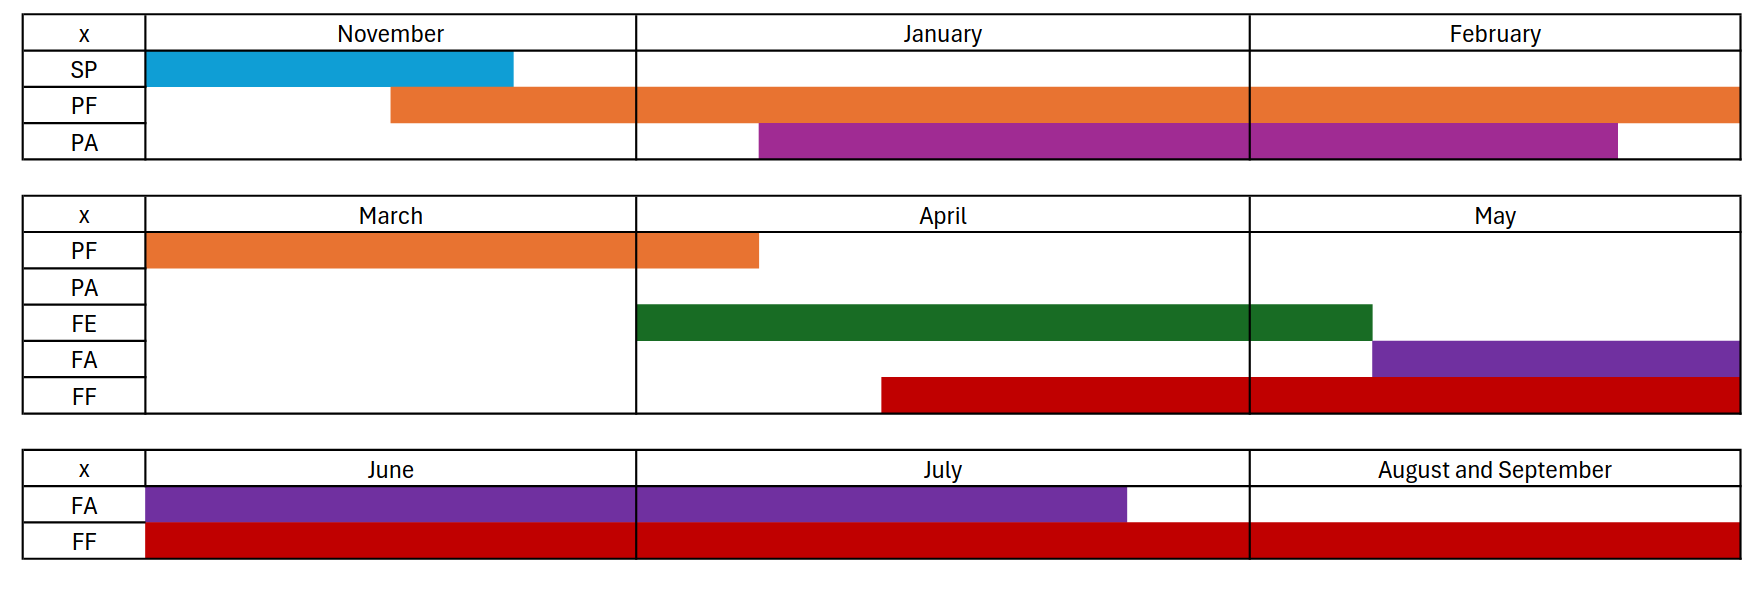
\includegraphics[width=\linewidth]{Figures/2Plan.png}
  \caption{Our plan until the second progression review.}
\end{figure}

Completeness of \OL{} we reserve for a later stage of the project.

%% ----------------------------------------------------------------
%% Conclusions.tex
%% ---------------------------------------------------------------- 
\section{Conclusions} \label{section: Conclusions}

\TODO


%\begin{lstlisting}[caption=Listing of what an example listing would be like]
%This is a test listing

%The test listing has serveral lines
%to show how the listings
%will be displayed
%\end{lstlisting}
%\appendix
%\include{AppendixA}
%\backmatter
%\chapter{Glossary [if relevant]}
\bibliographystyle{plainnat}
\bibliography{UOS}
%\chapter{Bibliography}
%To use bibliography as well as the references section use the \texttt{multibbl} package.
%\chapter{Index [if relevant]}
\end{document}
%% ----------------------------------------------------------------
